\documentclass[12pt, aspectratio=169]{beamer}

\usepackage{ctex}
\usepackage{amsmath, amssymb, amsfonts}
\usepackage{graphicx}
\usepackage{booktabs}
\usepackage{tikz}
\usepackage{multicol}
\usepackage{array}

% 主题设置
\usetheme{Madrid}
\usecolortheme{default}
\usefonttheme{professionalfonts} % 保持数学字体美观

% 标题信息
\title{第四章：单层神经网络 - 回归模型术语解析与习题}
\subtitle{从最小二乘法到贝叶斯推断}
\author{《深度学习基础》课程小组}
\date{\today}

% 自定义命令
\newcommand{\vect}[1]{\mathbf{#1}}
\newcommand{\mat}[1]{\mathbf{#1}}
\newcommand{\R}{\mathbb{R}}
\newcommand{\E}{\mathbb{E}}
\newcommand{\N}{\mathcal{N}}

\begin{document}

% 封面页
\begin{frame}
    \titlepage
\end{frame}

% 目录页
\begin{frame}{目录}
    \tableofcontents
\end{frame}

\section{单层网络-回归模型的知识图谱}
\begin{frame}
    \frametitle{单层网络-回归模型的知识图谱}
    \begin{center}
    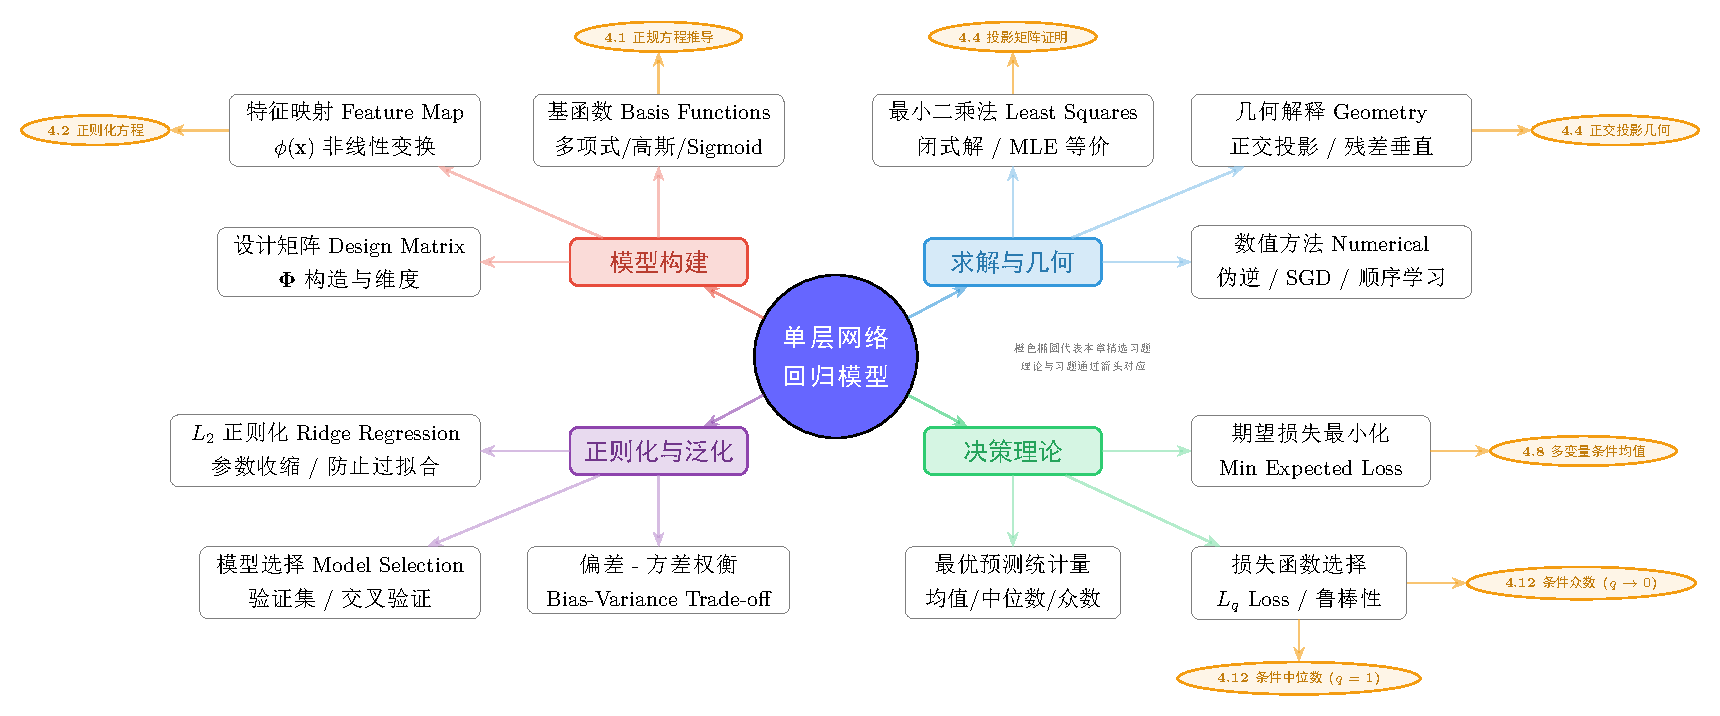
\includegraphics[width=0.95\textwidth]{ch04-graph.pdf}
    \end{center}
\end{frame}

\section{模型构建与基础}

% 1. Linear Regression
\begin{frame}{线性回归 (Linear Regression)}
    \begin{itemize}
        \item \textbf{定义}：一种基本的统计学习方法，用于建模输入变量 $\vect{x}$ 与连续目标变量 $t$ 之间的线性关系。
        \item \textbf{模型形式}：
        $$ y(\vect{x}, \vect{w}) = w_0 + \sum_{i=1}^D w_i x_i = \vect{w}^T \tilde{\vect{x}} $$
        其中 $\tilde{\vect{x}}$ 是增广输入向量（包含 $x_0=1$）。
        \item \textbf{在神经网络中的位置}：
        \begin{itemize}
            \item 单层网络的最基本形式。
            \item 如果没有激活函数（或激活函数为恒等函数），输出层即为线性回归。
        \end{itemize}
        \item \textbf{目标}：找到权重 $\vect{w}$，使得预测值 $y(\vect{x}, \vect{w})$ 尽可能接近真实值 $t$。
    \end{itemize}
\end{frame}

% 2. Basis functions
\begin{frame}{基函数 (Basis Functions)}
    \begin{itemize}
        \item \textbf{动机}：标准线性回归只能拟合线性关系。为了拟合非线性数据，我们将输入 $\vect{x}$ 通过一组非线性函数变换。
        \item \textbf{广义线性回归模型}：
        $$ y(\vect{x}, \vect{w}) = w_0 + \sum_{j=1}^M w_j \phi_j(\vect{x}) = \vect{w}^T \boldsymbol{\phi}(\vect{x}) $$
        其中 $\boldsymbol{\phi}(\vect{x}) = [\phi_1(\vect{x}), \dots, \phi_M(\vect{x})]^T$ 是基函数向量。
        \item \textbf{关键点}：
        \begin{itemize}
            \item 模型关于参数 $\vect{w}$ 仍然是\textbf{线性}的（这是“线性回归”名称的由来）。
            \item 关于输入 $\vect{x}$ 可以是非线性的。
        \end{itemize}
        \item \textbf{常见基函数}：多项式基、高斯基、Sigmoid基。
    \end{itemize}
\end{frame}

% 3. Feature extraction
\begin{frame}{特征提取 (Feature Extraction)}
    \begin{itemize}
        \item \textbf{定义}：将原始输入数据 $\vect{x}$ 转换为新的表示形式 $\boldsymbol{\phi}(\vect{x})$ 的过程。
        \item \textbf{与基函数的关系}：
        \begin{itemize}
            \item 基函数 $\phi_j(\vect{x})$ 的输出即为提取出的新\textbf{特征}。
            \item 这一层通常被称为神经网络的“隐藏层”或“特征层”。
        \end{itemize}
        \item \textbf{目的}：
        \begin{itemize}
            \item 将数据映射到一个更高维或更具判别力的空间，使得在该空间中数据呈现线性可分或线性可回归的特性。
            \item 例如：将一维 $x$ 映射为 $(x, x^2, x^3)$，从而可以用平面拟合曲线。
        \end{itemize}
        \item \textbf{现代视角}：在深度学习中，特征提取通常是自动学习的（通过反向传播），而在传统单层网络中，基函数往往是预先固定的。
    \end{itemize}
\end{frame}

% 4. Likelihood function
\begin{frame}{似然函数 (Likelihood Function)}
    \begin{itemize}
        \item \textbf{概率视角}：假设目标值 $t$ 由确定性函数 $y(\vect{x}, \vect{w})$ 加上高斯噪声 $\epsilon$ 生成：
        $$ t = y(\vect{x}, \vect{w}) + \epsilon, \quad \epsilon \sim \N(0, \beta^{-1}) $$
        \item \textbf{条件分布}：
        $$ p(t|\vect{x}, \vect{w}, \beta) = \N(t | y(\vect{x}, \vect{w}), \beta^{-1}) $$
        \item \textbf{似然函数}：给定数据集 $D = \{(\vect{x}_n, t_n)\}_{n=1}^N$，参数的似然函数为所有数据点概率的乘积：
        $$ L(\vect{w}, \beta) = \prod_{n=1}^N \N(t_n | \vect{w}^T \boldsymbol{\phi}(\vect{x}_n), \beta^{-1}) $$
        \item \textbf{作用}：最大化似然函数 (MLE) 等价于最小化平方和误差函数。
    \end{itemize}
\end{frame}

\section{参数求解与几何解释}

% 5. Moore–Penrose pseudo-inverse
\begin{frame}{Moore–Penrose 伪逆 (Moore–Penrose Pseudo-inverse)}
    \begin{itemize}
        \item \textbf{背景}：线性回归的最小二乘解需要求解正规方程 (Normal Equation)：
        $$ (\boldsymbol{\Phi}^{\mathrm{T}} \boldsymbol{\Phi}) \vect{w} = \boldsymbol{\Phi}^{\mathrm{T}} \vect{t} $$
        其中 $\boldsymbol{\Phi}$ 是设计矩阵 (Design Matrix)。
        \item \textbf{问题}：当 $\boldsymbol{\Phi}^T \boldsymbol{\Phi}$ 不可逆时（例如特征数多于样本数，或特征间存在多重共线性），无法直接求逆。
        \item \textbf{解决方案}：使用 Moore–Penrose 伪逆 
        $\boldsymbol{\Phi}^\dagger = (\boldsymbol{\Phi}^{\mathrm{T}}\boldsymbol{\Phi})^{-1}\boldsymbol{\Phi}^{\mathrm{T}}$.
        \item \textbf{解析解}：
        $$ \vect{w}_{\text{ML}} = \boldsymbol{\Phi}^\dagger \vect{t} $$
        \item \textbf{性质}：即使矩阵不是方阵或奇异，伪逆也能给出一个最小范数的最小二乘解。
    \end{itemize}
\end{frame}

% 6. Geometry of least squares
\begin{frame}{最小二乘法的几何解释 (Geometry of Least Squares)}
    \begin{itemize}
        \item \textbf{向量空间}：
        \begin{itemize}
            \item 目标向量 $\vect{t}$ 位于 $N$ 维空间中。
            \item 设计矩阵 $\boldsymbol{\Phi}$ 的列向量张成一个子空间 $\mathcal{S}$。
        \end{itemize}
        \item \textbf{投影}：
        \begin{itemize}
            \item 最小二乘法的目标是找到 $\mathcal{S}$ 中的一个向量 $\vect{y} = \boldsymbol{\Phi}\vect{w}$，使其与 $\vect{t}$ 的距离（欧几里得距离）最小。
            \item 这个最优的 $\vect{y}$ 正是 $\vect{t}$ 在子空间 $\mathcal{S}$ 上的\textbf{正交投影}。
        \end{itemize}
        \item \textbf{残差}：误差向量 $\vect{e} = \vect{t} - \boldsymbol{\Phi}\vect{w}$ 垂直于子空间 $\mathcal{S}$（即垂直于 $\boldsymbol{\Phi}$ 的所有列）。
        \item \item 数学表达：$\boldsymbol{\Phi}^{\mathrm{T}} (\vect{t} - \boldsymbol{\Phi}\vect{w}) = \vect{0}$，这正是正规方程。
    \end{itemize}
\end{frame}

% 7. Sequential learning
\begin{frame}{顺序学习 (Sequential Learning)}
    \begin{itemize}
        \item \textbf{定义}：也称为在线学习 (Online Learning)。模型数据点逐个（或小批量）到达，每收到一个新数据就更新一次参数，而不是等待所有数据收集完毕（批处理）。
        \item \textbf{优势}：
        \begin{itemize}
            \item 适用于数据流场景或内存受限的情况。
            \item 能够适应数据分布随时间变化的情况（概念漂移）。
        \end{itemize}
        \item \textbf{算法示例}：
        \begin{itemize}
            \item 递归最小二乘法 (RLS)。
            \item 随机梯度下降 (SGD)。
        \end{itemize}
        \item \textbf{更新规则}：$\vect{w}_{\mathrm{new}} = \vect{w}_{\mathrm{old}} - \eta \nabla E_n(\vect{w}_{\mathrm{old}})$，其中 $E_n$ 是当前单个样本的误差。
    \end{itemize}
\end{frame}

% 8. Stochastic gradient descent
\begin{frame}{随机梯度下降 (Stochastic Gradient Descent, SGD)}
    \begin{itemize}
        \item \textbf{对比}：
        \begin{itemize}
            \item \textbf{批梯度下降}：每次更新遍历所有 $N$ 个样本计算总梯度。计算量大，收敛稳但慢。
            \item \textbf{SGD}：每次更新仅基于\textbf{一个}随机选取的样本 $(\vect{x}_n, t_n)$。
        \end{itemize}
        \item \textbf{更新公式}：
        $$ \vect{w}^{(\tau+1)} = \vect{w}^{(\tau)} - \eta \nabla E_n(\vect{w}^{(\tau)}) $$
        其中 $E_n(\vect{w}) = \frac{1}{2}(y(\vect{x}_n, \vect{w}) - t_n)^2$. 
        \item \textbf{特点}：
        \begin{itemize}
            \item 计算速度快，可立即响应新数据。
            \item 路径具有随机性（在极小值附近震荡），需要逐渐减小学习率 $\eta$ 以保证收敛。
        \end{itemize}
    \end{itemize}
\end{frame}

\section{正则化与模型选择}

% 9. Regularized least squares
\begin{frame}{正则化最小二乘法 (Regularized Least Squares)}
    \begin{itemize}
        \item \textbf{问题}：普通最小二乘法容易过拟合（Overfitting），特别是当基函数过多或数据噪声大时，权重 $\vect{w}$ 会变得非常大。
        \item \textbf{方法}：在误差函数中加入惩罚项（正则化项）。
        $$ E(\vect{w}) = \frac{1}{2}\sum_{n=1}^N (y(\vect{x}_n, \vect{w}) - t_n)^2 + \frac{\lambda}{2} \|\vect{w}\|^2 $$
        \item \textbf{$L_2$ 正则化}：上述公式称为岭回归 (Ridge Regression)。
        \item \textbf{效果}：
        \begin{itemize}
            \item 限制权重的大小，使模型更平滑。
            \item $\lambda$ 控制惩罚力度：$\lambda$ 越大，权重越趋近于 0。
        \end{itemize}
        \item \textbf{解析解}：$\vect{w} = (\boldsymbol{\Phi}^{\mathrm{T}} \boldsymbol{\Phi} + \lambda \mat{I})^{-1} \boldsymbol{\Phi}^{\mathrm{T}} \vect{t}$。加入 $\lambda \mat{I}$ 保证了矩阵可逆。
    \end{itemize}
\end{frame}

% 10. Parameter shrinkage method
\begin{frame}{参数收缩法 (Parameter Shrinkage Method)}
    \begin{itemize}
        \item \textbf{定义}：正则化技术的一种统称，因为其效果是将参数估计值向零（或某个先验均值）“收缩” (Shrink)。
        \item \textbf{常见类型}：
        \begin{itemize}
            \item \textbf{Ridge Regression ($L_2$)}：$\lambda \sum w_i^2$。使权重变小但不为零，适合处理多重共线性。
            \item \textbf{Lasso ($L_1$)}：$\lambda \sum |w_i|$。倾向于产生稀疏解（部分权重精确为 0），具有特征选择功能。
        \end{itemize}
        \item \textbf{贝叶斯解释}：
        \begin{itemize}
            \item $L_2$ 正则化等价于假设权重服从高斯先验 $p(\vect{w}) = \N(\vect{0}, \alpha^{-1}\mat{I})$ 时的最大后验估计 (MAP)。
            \item $L_1$ 正则化等价于假设权重服从拉普拉斯先验。
        \end{itemize}
    \end{itemize}
\end{frame}

% 11. The Bias–Variance Trade-off
\begin{frame}{偏差 - 方差权衡 (The Bias–Variance Trade-off)}
    \begin{itemize}
        \item \textbf{期望预测误差分解}：对于新的输入 $\vect{x}$，期望平方误差可以分解为三部分：
        $$ \E[(t - y(\vect{x}))^2] = (\text{Bias})^2 + \text{Variance} + \text{Noise} $$
        \item \textbf{偏差 (Bias)}：
        \begin{itemize}
            \item 模型预测的平均值与真实值之间的差异。
            \item 高偏差意味着模型太简单（欠拟合），无法捕捉数据的内在规律。
        \end{itemize}
        \item \textbf{方差 (Variance)}：
        \begin{itemize}
            \item 模型预测值在不同训练集上的波动程度。
            \item 高方差意味着模型太复杂（过拟合），过度记住了训练数据的噪声。
        \end{itemize}
        \item \textbf{权衡}：
        \begin{itemize}
            \item 增加模型复杂度 $\to$ 偏差降低，方差升高。
            \item 减少模型复杂度（或增加正则化） $\to$ 偏差升高，方差降低。
            \item 目标是找到总误差最小的平衡点。
        \end{itemize}
    \end{itemize}
\end{frame}

\section{决策理论与贝叶斯视角}

% 12. Decision theory
\begin{frame}{决策理论 (Decision Theory)}
    \begin{itemize}
        \item \textbf{核心思想}：在回归问题中，我们需要根据输入 $\vect{x}$ 做出一个预测 $y(\vect{x})$，以最小化预期的损失。
        \item \textbf{损失函数}：常用平方损失 $L(t, y) = (y - t)^2$。
        \item \textbf{期望损失最小化}：
        $\displaystyle \min_{y(\vect{x})} \E[L] = \min_{y(\vect{x})} \iint (y(\vect{x}) - t)^2 p(\vect{x}, t) \, dt \, d\vect{x} $
        \item \textbf{结论}：
            对于平方损失，最优预测 $y^*(\vect{x})$ 是目标变量的\textbf{条件期望}：
            $$ y^*(\vect{x}) = \E_t[t|\vect{x}] = \int t \, p(t|\vect{x}) \, dt $$
            这就是为什么我们在回归中通常试图逼近条件均值。
        \item \textbf{其他损失}：若使用绝对值损失 $|y-t|$，最优解为条件中位数；若使用 $0-1$ 损失（离散化），最优解为条件众数。
    \end{itemize}
\end{frame}

% 13. Predictive distribution
\begin{frame}{预测分布 (Predictive Distribution)}
    \begin{itemize}
        \item \textbf{超越点估计}：传统的回归只给出一个预测值 $y(\vect{x})$。贝叶斯方法则给出一个完整的概率分布 $p(t|\vect{x}, D)$，反映了预测的不确定性。
        \item \textbf{构成}：
        $$ p(t|\vect{x}, D) = \int p(t|\vect{x}, \vect{w}) p(\vect{w}|D) \, d\vect{w} $$
        \begin{itemize}
            \item $p(t|\vect{x}, \vect{w})$：给定参数的噪声模型（通常是高斯）。
            \item $p(\vect{w}|D)$：参数的后验分布（反映了我们对权重的不确定度）。
        \end{itemize}
        \item \textbf{结果}：
        \begin{itemize}
            \item 预测分布通常也是一个高斯分布。
            \item 其方差包含两部分：数据本身的噪声方差 + 参数不确定性带来的方差。
            \item 在训练数据稀缺的区域，预测分布的方差会变大（模型表示“我不确定”）。
        \end{itemize}
    \end{itemize}
\end{frame}

% 补充：Sum-of-Squares Error (为了完整性)
\begin{frame}{平方和误差函数 (Sum-of-Squares Error Function)}
    \begin{itemize}
        \item \textbf{定义}：衡量模型预测值与真实值之间差异的最常用指标。
        $$ E(\vect{w}) = \frac{1}{2} \sum_{n=1}^N \left( y(\vect{x}_n, \vect{w}) - t_n \right)^2 $$
        \item \textbf{系数 1/2}：为了方便求导后消去平方项的系数 2，不影响优化结果。
        \item \textbf{与似然的关系}：
        \begin{itemize}
            \item 在高斯噪声假设下，最大化对数似然函数 $\ln L$ 等价于最小化 $E(\vect{w})$。
            \item 这建立了概率模型与经典最小二乘法之间的桥梁。
        \end{itemize}
        \item \textbf{局限性}：对异常值（Outliers）敏感，因为误差被平方放大了。
    \end{itemize}
\end{frame}

% 补充：Design Matrix (为了完整性)
\begin{frame}{设计矩阵 (Design Matrix)}
    \begin{itemize}
        \item \textbf{定义}：将数据集中的所有输入经过基函数变换后排列成的矩阵。
        $$ \boldsymbol{\Phi} = \begin{pmatrix} 
        \phi_0(\vect{x}_1) & \phi_1(\vect{x}_1) & \cdots & \phi_M(\vect{x}_1) \\
        \phi_0(\vect{x}_2) & \phi_1(\vect{x}_2) & \cdots & \phi_M(\vect{x}_2) \\
        \vdots & \vdots & \ddots & \vdots \\
        \phi_0(\vect{x}_N) & \phi_1(\vect{x}_N) & \cdots & \phi_M(\vect{x}_N)
        \end{pmatrix} $$
        \item \textbf{维度}：$N \times M$ （$N$ 个样本，$M$ 个基函数/特征）。
        \item \textbf{作用}：
        \begin{itemize}
            \item 将非线性的基函数变换转化为线性的矩阵运算。
            \item 模型预测向量可简洁地写为 $\vect{y} = \boldsymbol{\Phi}\vect{w}$。
            \item 是推导正规方程和几何解释的核心对象。
        \end{itemize}
    \end{itemize}
\end{frame}

% 结束页
\begin{frame}{总结}
    \begin{itemize}
        \item \textbf{建模}：通过\textbf{基函数}和\textbf{特征提取}，单层网络可以处理非线性回归问题。
        \item \textbf{求解}：\textbf{最小二乘法}及其几何解释提供了闭式解，而\textbf{SGD}和\textbf{顺序学习}适应了大规模数据。
        \item \textbf{泛化}：\textbf{正则化}和\textbf{参数收缩}是防止过拟合、平衡\textbf{偏差与方差}的关键手段。
        \item \textbf{理论基石}：\textbf{决策理论}证明了最小二乘对应于条件期望，而\textbf{预测分布}则提供了更丰富的不确定性信息。
        \item 这些概念共同构成了现代机器学习和深度学习回归任务的理论基础。
    \end{itemize}
\end{frame}


\section{五个习题}
% -----------------------------------------------------------
% 习题 4.1: 多项式回归的正规方程
% -----------------------------------------------------------
\begin{frame}{习题 4.1 $(\star)$: 多项式回归的正规方程}
    \framesubtitle{平方和误差函数的最小化}
    % \textbf{问题描述：}
    考虑由下式给出的平方和误差函数：
    %\begin{equation}
    $\displaystyle
    E(\mathbf{w}) = \frac{1}{2} \sum_{n=1}^{N} \left[ y(x_n,\mathbf{w})-t_n \right]^2
    $
    %\end{equation}

    其中模型 $y(x, \mathbf{w})$ 为 $M$ 阶多项式：
    %\begin{equation}
    $\displaystyle y(x, \mathbf{w}) = w_0 + w_1x + w_2x^2 + \cdots + w_Mx^M 
    $
    %\end{equation}

    \vspace{0.5em}
    % \textbf{任务：}
    证明最小化该误差函数的系数 $\mathbf{w} = \{w_i\}$ 由以下线性方程组的解给出：
    \begin{equation}
        \sum_{j=0}^{M} A_{ij} w_j = T_i, \quad (i=0,1,\dots,M)
    \end{equation}
    其中系数定义为：
    %\begin{align}
    $\displaystyle
        A_{ij} = \sum_{n=1}^{N} (x_n)^{i+j}, \quad 
        T_i = \sum_{n=1}^{N} (x_n)^i t_n.
    $
    %\end{align}
    
    \vspace{0.5em}
    \footnotesize{提示：对 $E(\mathbf{w})$ 关于 $w_i$ 求偏导并令其为零。}
\end{frame}

% -----------------------------------------------------------
% 习题 4.2: 正则化回归
% -----------------------------------------------------------
\begin{frame}{习题 4.2 $(\star)$: 正则化回归}
    \framesubtitle{引入正则化项后的线性方程}
    % \textbf{问题描述：}
    现在考虑加入 $L_2$ 正则化项的误差函数：
    \begin{equation}
        \tilde{E} (\mathbf{w}) = \underbrace{\frac{1}{2}\sum_{n=1}^{N} \left[ y(x_n,\mathbf{w})-t_n \right]^2}_{\text{数据项}} + \underbrace{\frac{\lambda}{2} \lVert \mathbf{w} \rVert^2}_{\text{正则化项}}
    \end{equation}
    其中 $\lVert \mathbf{w} \rVert^2 = \mathbf{w}^\mathrm{T}\mathbf{w} = \sum_{i=0}^M w_i^2$。
    
    \vspace{0.5em}
    % \textbf{任务：}
    写出类似于习题 4.1 中的一组耦合线性方程，这些方程由最小化 $\tilde{E}(\mathbf{w})$ 的系数 $w_i$ 所满足。
    正则化参数 $\lambda$ 如何改变矩阵 $A_{ij}$ 的对角线元素？
    
\end{frame}

% -----------------------------------------------------------
% 习题 4.4: 几何解释与投影
% -----------------------------------------------------------
\begin{frame}{习题 4.4 $(\star\star\star)$: 几何解释与投影}
    \framesubtitle{最小二乘法的几何意义}
    
    \textbf{第一部分：投影矩阵。}
    证明矩阵
    \begin{equation}
        \mathbf{P} = \boldsymbol{\Phi}(\boldsymbol{\Phi}^{\mathrm{T}}\boldsymbol{\Phi})^{-1}\boldsymbol{\Phi}^{\mathrm{T}}
    \end{equation}
    是将任意向量 $\mathbf{v}$ 投影到由设计矩阵 $\boldsymbol{\Phi}$ 的列张成的空间 $\mathcal{S}$ 上的投影算子。

    (需验证 $\mathbf{P}^2=\mathbf{P}$ 且 $\mathbf{P}^\mathrm{T}=\mathbf{P}$)
    
    \vspace{1em}
    \textbf{第二部分：正交投影。}
    利用上述结果证明，最小二乘解
    \begin{equation}
        \mathbf{w}_{ML} = (\boldsymbol{\Phi}^{\mathrm{T}}\boldsymbol{\Phi})^{-1}\boldsymbol{\Phi}^{\mathrm{T}} \mathbf{t}
    \end{equation}
    对应的预测向量 $\mathbf{y} = \boldsymbol{\Phi}\mathbf{w}_{ML}$ 恰好是目标向量 $\mathbf{t}$ 到流形 $\mathcal{S}$ 上的\textbf{正交投影}。
    
    % \begin{center}
    %     \includegraphics[width=0.6\textwidth]{example-image-a} % 此处可替换为教材图4.3
    %     \vspace{-1em}
    %     \scriptsize{示意图：$\mathbf{t}$ 分解为投影分量 $\mathbf{y}$ 和误差分量 $\mathbf{t}-\mathbf{y}$}
    % \end{center}
\end{frame}

% -----------------------------------------------------------
% 习题 4.8: 多变量回归的期望损失
% -----------------------------------------------------------
\begin{frame}{习题 4.8 $(\star)$: 多变量回归的期望损失}
    \framesubtitle{从单变量到多变量的条件期望}
    
    \textbf{背景：}
    单变量平方损失的最小化解是条件期望 $\mathbb{E}[t|\mathbf{x}]$。
    
    \textbf{推广：}
    考虑由向量 $\mathbf{t}$ 描述的多个目标变量，其期望损失为：
    \begin{equation}
        \mathbb{E}[L] = \iint \lVert\mathbf{f}(\mathbf{x}) - \mathbf{t}\rVert^2 p(\mathbf{x}, \mathbf{t}) \,\mathrm{d}\mathbf{x}\,\mathrm{d}\mathbf{t}
    \end{equation}
    
    % \vspace{0.5em}
    \textbf{任务：}
    使用变分法（或对 $\mathbf{f}(\mathbf{x})$ 直接求导），证明使该期望损失最小化的函数 $\mathbf{f}(\mathbf{x})$ 由下式给出：
    \begin{equation}
        \mathbf{f}(\mathbf{x}) = \mathbb{E}_{\mathbf{t}}[\mathbf{t}|\mathbf{x}]
    \end{equation}
    
    % \vspace{0.5em}
    \begin{alertblock}{结论}
        即使在多输出情况下，最小化均方误差的最优预测仍然是目标向量的\textbf{条件均值}。
    \end{alertblock}
\end{frame}

% -----------------------------------------------------------
% 习题 4.12: Lq 损失与鲁棒回归
% -----------------------------------------------------------
\begin{frame}{习题 4.12 $(\star\star)$: Lq 损失与鲁棒回归}
    \framesubtitle{不同 $q$ 值下的最优解}
    
    考虑 $L_q$ 损失函数下的期望损失：
    \begin{equation}
        \mathbb{E}[L_q] = \iint \lvert f(\mathbf{x}) - t\rvert^q p(\mathbf{x}, t) \,\mathrm{d}\mathbf{x}\,\mathrm{d}t
    \end{equation}
    
    % \textbf{任务：}
    \begin{enumerate}
        \item 为了最小化 $\mathbb{E}[L_q]$, 写出 $y(\mathbf{x})$ 必须满足的一般条件。
        \item \textbf{当 $q=1$ 时：}
        证明该解代表\textbf{条件中位数}。即 $y(\mathbf{x})$ 使得：
        \[ P(t < y(\mathbf{x}) | \mathbf{x}) = P(t \ge y(\mathbf{x}) | \mathbf{x}) = 0.5 \]
        \item \textbf{当 $q \to 0$ 时：}
        证明最小期望损失由\textbf{条件众数}给出。即 $y(\mathbf{x})$ 等于使条件概率密度 $p(t|\mathbf{x})$ 最大化的 $t$ 值。
    \end{enumerate}
    
    \vspace{0.5em}
    \footnotesize{讨论：这说明不同的损失函数对应着对目标分布不同统计特性的估计。}
\end{frame}


\end{document}
